% CS631 Advanced Programming in the UNIX Environment
% Author: Jan Schaumann <jschauma@netmeister.org>
\special{! TeXDict begin /landplus90{true}store end }

\documentclass[xga]{xdvislides}
\usepackage[landscape]{geometry}
\usepackage{graphics}
\usepackage{graphicx}
\usepackage{colordvi}

\begin{document}
\setfontphv

%%% Headers and footers
\lhead{\slidetitle}
\chead{CS631 - Advanced Programming in the UNIX Environment}
\rhead{\relax}
\lfoot{\Gray{Lecture 02: File I/O, File Sharing}}
\cfoot{\relax}
\rfoot{\Gray{\today}}

\vspace*{\fill}
\begin{center}
	\Hugesize
		CS631 - Advanced Programming in the UNIX Environment\\ [1em]
		File I/O, File Sharing
	\hspace*{5mm}\blueline\\ [1em]
	\Normalsize
		Department of Computer Science\\
		Stevens Institute of Technology\\
		Jan Schaumann\\
		\verb+jschauma@stevens.edu+\\
		\verb+https://stevens.netmeister.org/631/+
\end{center}
\vspace*{\fill}

\subsection{Recall {\tt simple-cat.c} from last week...}
\begin{verbatim}
int main(int argc, char **argv) {
        int n;
        char buf[BUFFSIZE];

        while ((n = read(STDIN_FILENO, buf, BUFFSIZE)) > 0) {
                if (write(STDOUT_FILENO, buf, n) != n) {
                        fprintf(stderr, "write error\n");
                        exit(1);
                }
        }
        if (n < 0) {
                fprintf(stderr, "read error\n");
                exit(1);
        }

        return(0);
}
\end{verbatim}

\subsection{Warm-up exercise}
Write a program that:
\begin{itemize}
	\item prints the value of {\tt STDIN\_FILENO},
		{\tt STDOUT\_FILENO}, {\tt STDERR\_FILENO}
	\item prints the value of the file descriptors
		referenced via the {\tt stdin}, {\tt
		stdout}, {\tt stderr} streams
	\item {\tt open(2)}'s a file, then prints the
		value of that file descriptor
	\item {\tt fopen(3)}'s a file, then prints
		the value of the file descriptor
		referenced via that stream
\end{itemize}

What results do you expect?

\subsection{Let's look at the file descriptors.}
\vspace*{\fill}
\begin{center}
\Huge
\verb+fds.c+
\normalsize
\end{center}
\vspace*{\fill}



%\subsection{Shell Command-Line Processing}
%\begin{center}
%\Huge
%\begin{verbatim}
%$ cc -Wall argv.c
%$ ./a.out
%$ ./a.out *.c
%$ ./a.out *.none
%$ ./a.out *.[1c]
%$ ./a.out "*.c"
%$ ./a.out $USER
%$ ./a.out "$(echo *.1)"
%$ ./a.out {foo,bar,baz}.whatever
%$ ./a.out {1..5}
%$ ./a.out {1..5}{a..f}
%\end{verbatim}
%\normalsize
%\vspace{.25in}
%See also:
%\verb+http://is.gd/Ydgywd+ and \verb+http://is.gd/iZa9rC+
%\end{center}
%
\subsection{File Descriptors}
\begin{itemize}
	\item A {\em file descriptor} (or {\em file handle}) is a small,
		non-negative integer which identifies a file to the kernel.
\end{itemize}


\subsection{File Descriptors}
\begin{itemize}
	\item A {\em file descriptor} (or {\em file handle}) is a small,
		non-negative integer which identifies a file to the kernel.
	\item Traditionally, {\tt stdin}, {\tt stdout} and {\tt stderr}
		are 0, 1 and 2 respectively.
\end{itemize}

\subsection{File Descriptors}
\begin{itemize}
	\item A {\em file descriptor} (or {\em file handle}) is a small,
		non-negative integer which identifies a file to the kernel.
	\item Traditionally, {\tt stdin}, {\tt stdout} and {\tt stderr}
		are 0, 1 and 2 respectively.
\end{itemize}
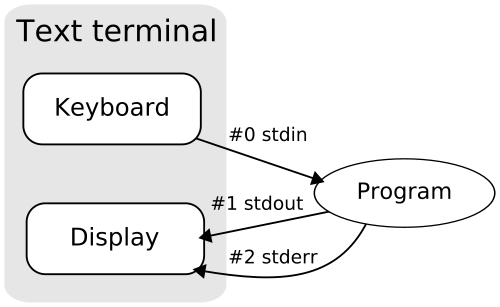
\includegraphics[scale=0.6,angle=-90]{pics/stdstreams.eps}

\subsection{File Descriptors}
\begin{itemize}
	\item A {\em file descriptor} (or {\em file handle}) is a small,
		non-negative integer which identifies a file to the kernel.
	\item Traditionally, {\tt stdin}, {\tt stdout} and {\tt stderr}
		are 0, 1 and 2 respectively.
\end{itemize}
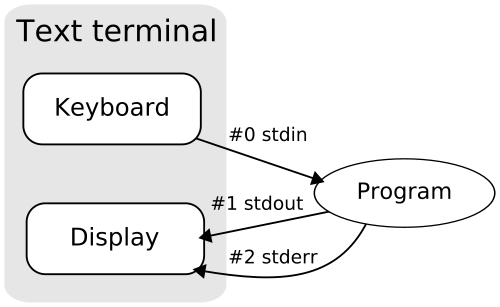
\includegraphics[scale=0.61,angle=-90]{pics/stdstreams.eps}
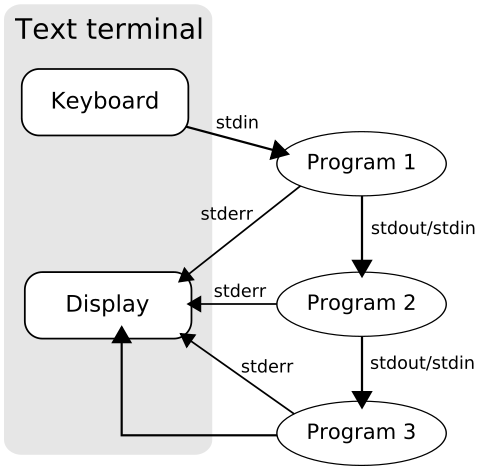
\includegraphics[scale=0.53,angle=-90]{pics/pipeline.eps}



\subsection{File Descriptors}
\begin{itemize}
	\item A {\em file descriptor} (or {\em file handle}) is a small,
		non-negative integer which identifies a file to the kernel.
	\item Traditionally, {\tt stdin}, {\tt stdout} and {\tt stderr}
		are 0, 1 and 2 respectively.
	\item Relying on ``magic numbers'' is Bad\texttrademark.  Use {\tt
		STDIN\_FILENO}, {\tt STDOUT\_FILENO} and {\tt STDERR\_FILENO}.
\end{itemize}

\subsection{File Descriptors}
\begin{itemize}
	\item A {\em file descriptor} (or {\em file handle}) is a small,
		non-negative integer which identifies a file to the kernel.
	\item Traditionally, {\tt stdin}, {\tt stdout} and {\tt stderr}
		are 0, 1 and 2 respectively.
	\item Relying on ``magic numbers'' is Bad\texttrademark.  Use {\tt
		STDIN\_FILENO}, {\tt STDOUT\_FILENO} and {\tt STDERR\_FILENO}.
	\item All resources are finite.  So are file descriptors.  So... how many can you have?
\end{itemize}


\subsection{File Descriptors}
\begin{itemize}
	\item A {\em file descriptor} (or {\em file handle}) is a small,
		non-negative integer which identifies a file to the kernel.
	\item Traditionally, {\tt stdin}, {\tt stdout} and {\tt stderr}
		are 0, 1 and 2 respectively.
	\item Relying on ``magic numbers'' is Bad\texttrademark.  Use {\tt
		STDIN\_FILENO}, {\tt STDOUT\_FILENO} and {\tt STDERR\_FILENO}.
	\item All resources are finite.  So are file descriptors.  So... how many can you have?
\end{itemize}

\addvspace{.5in}
\begin{center}
\Huge
\verb+openmax.c+
\normalsize
\end{center}

\vspace*{\fill}
See also: \verb+https://en.wikipedia.org/wiki/File_descriptor+

\subsection{Standard I/O}
Basic File I/O: almost all UNIX file I/O can be
performed using these five functions:
\begin{itemize}
	\item {\tt open(2)}
	\item {\tt close(2)}
	\item {\tt lseek(2)}
	\item {\tt read(2)}
	\item {\tt write(2)}
\end{itemize}
\vspace{.25in}
Processes may want to share recources.  This requires us to look at:
\begin{itemize}
	\item atomicity of these operations
	\item file sharing
	\item manipulation of file descriptors
\end{itemize}

\subsection{{\tt creat(2)}}
\small
\setlength{\unitlength}{1mm}
\begin{center}
	\begin{picture}(230,25)
		\thinlines
		\put(0,0){\framebox(210,25){}}
		\put(10,20){{\tt \#include <fcntl.h>}}
		\put(10,10){{\tt int creat(const char *{\em pathname}, mode\_t {\em mode});}}
		\put(145,3){Returns:  file descriptor if OK, -1 on error}
	\end{picture}
\end{center}
\begin{center}

\includegraphics[width=540px]{pics/creation.eps} \\
\small
\verb+https://is.gd/x4KPa2+
\end{center}
\Normalsize

\subsection{{\tt creat(2)}}
\small
\setlength{\unitlength}{1mm}
\begin{center}
	\begin{picture}(230,25)
		\thinlines
		\put(0,0){\framebox(210,25){}}
		\put(10,20){{\tt \#include <fcntl.h>}}
		\put(10,10){{\tt int creat(const char *{\em pathname}, mode\_t {\em mode});}}
		\put(145,3){Returns:  file descriptor if OK, -1 on error}
	\end{picture}
\end{center}
\Normalsize
\vspace{.5in}
{\bf This interface is made obsolete by {\tt open(2)}.} \\

\subsection{{\tt open(2)}}
\small
\setlength{\unitlength}{1mm}
\begin{center}
	\begin{picture}(230,25)
		\thinlines
		\put(0,0){\framebox(210,25){}}
		\put(10,20){{\tt \#include <fcntl.h>}}
		\put(10,12){{\tt int open(const char *{\em pathname}, int {\em oflag}, ... /* mode\_t {\em mode} */ );}}
		\put(145,3){Returns:  file descriptor if OK, -1 on error}
	\end{picture}
\end{center}
\vspace{.25in}
\Normalsize
{\em oflag} must be one (and only one) of:
\small
\begin{itemize}
	\item {\tt O\_RDONLY} -- Open for reading only
	\item {\tt O\_WRONLY} -- Open for writing only
	\item {\tt O\_RDWR} -- Open for reading and writing
\end{itemize}
\vspace{.25in}
\Normalsize
and may be OR'd with any of these:
\small
\begin{itemize}
	\item {\tt O\_APPEND} -- Append to end of file for each write
	\item {\tt O\_CREAT} -- Create the file if it doesn't exist. Requires
		{\em mode} argument
	\item {\tt O\_EXCL} -- Generate error if {\tt O\_CREAT} and file
		already exists. (atomic)
	\item {\tt O\_TRUNC} -- If file exists and successfully open in
		{\tt O\_WRONLY} or {\tt O\_RDWR}, make length = 0
	\item {\tt O\_NOCTTY} -- If pathname refers to a terminal device, do
		not allocate the device as a controlling terminal
	\item {\tt O\_NONBLOCK} -- If pathname refers to a FIFO, block special,
		or char special, set nonblocking mode (open and I/O)
	\item {\tt O\_SYNC} --  Each write waits for physical I/O to complete
\end{itemize}

\subsection{{\tt open(2)} variants}
\small
\setlength{\unitlength}{1mm}
\begin{center}
	\begin{picture}(230,28)
		\thinlines
		\put(0,0){\framebox(210,28){}}
		\put(10,23){{\tt \#include <fcntl.h>}}
		\put(10,15){{\tt int open(const char *{\em pathname}, int {\em oflag}, ... /* mode\_t {\em mode} */ );}}
		\put(10,10){{\tt int openat(int {\em dirfd}, const char *{\em pathname}, int {\em oflag}, ... /* mode\_t {\em mode} */ );}}
		\put(145,3){Returns:  file descriptor if OK, -1 on error}
	\end{picture}
\end{center}
\Normalsize
On some platforms additional {\em oflag}s may be supported:
\vspace{.2in}
\small
\begin{itemize}
	\item {\tt O\_EXEC} -- Open for execute only
	\item {\tt O\_SEARCH} -- Open for search only (applies to directories)
	\item {\tt O\_DIRECTORY} -- If path resolves to a non-directory file, fail and set errno to {\tt ENOTDIR}.
	\item {\tt O\_DSYNC} -- Wait for physical I/O for data, except
file attributes
	\item {\tt O\_RSYNC} -- Block read operations on any pending writes.
	\item {\tt O\_PATH} -- Obtain a file descriptor purely for fd-level operations. (Linux $>$2.6.36 only)
\end{itemize}
\vspace{.3in}
\Normalsize
{\tt openat(2)} is used to handle relative pathnames from different
working directories in an atomic fashion. % TOCTOU - time of check - time of use

\subsection{{\tt openat(2)}}
POSIX ({\tt https://is.gd/3hZ4EZ}) says: \\

{\em The purpose of the {\tt openat()} function is to enable
opening files in directories other than the current
working directory without exposure to race conditions.
Any part of the path of a file could be changed in
parallel to a call to {\tt open()}, resulting in unspecified
behavior. By opening a file descriptor for the target
directory and using the openat() function it can be
guaranteed that the opened file is located relative to
the desired directory. Some implementations use the
{\tt openat()} function for other purposes as well.}\\


Think of {\em specific} examples how this defeats TOCTOU
problems; write a Proof-of-Concept program to
illustrate.


\subsection{{\tt close(2)}}
\small
\setlength{\unitlength}{1mm}
\begin{center}
	\begin{picture}(230,25)
		\thinlines
		\put(0,0){\framebox(210,25){}}
		\put(10,20){{\tt \#include <unistd.h>}}
		\put(10,10){{\tt int close(int {\em fd});}}
		\put(145,3){Returns:  0 if OK, -1 on error}
	\end{picture}
\end{center}
\Normalsize
\vspace{.25in}
\begin{itemize}
	\item closing a filedescriptor releases any record locks on
		that file (more on that in future lectures)
	\item file descriptors not explicitly closed are closed by the kernel
		when the process terminates.
	\item to avoid leaking file descriptors, always {\tt close(2)}
		them within the same scope
\end{itemize}

\subsection{{\tt open(2)} and {\tt close(2)}}
\begin{center}
\Huge
\begin{verbatim}
openex.c
\end{verbatim}
\normalsize
\end{center}


\subsection{{\tt read(2)}}
\small
\setlength{\unitlength}{1mm}
\begin{center}
	\begin{picture}(230,25)
		\thinlines
		\put(0,0){\framebox(210,25){}}
		\put(10,20){{\tt \#include <unistd.h>}}
		\put(10,12){{\tt ssize\_t read(int {\em filedes}, void *{\em buff}, size\_t {\em nbytes} );}}
		\put(115,3){Returns:  number of bytes read, 0 if end of file, -1 on error}
	\end{picture}
\end{center}
\Normalsize
\begin{center}

\includegraphics[scale=0.6]{pics/reading.eps} \\
\small
\verb+https://is.gd/qI5r8E+
\end{center}
\Normalsize


\subsection{{\tt read(2)}}
\small
\setlength{\unitlength}{1mm}
\begin{center}
	\begin{picture}(230,25)
		\thinlines
		\put(0,0){\framebox(210,25){}}
		\put(10,20){{\tt \#include <unistd.h>}}
		\put(10,12){{\tt ssize\_t read(int {\em filedes}, void *{\em buff}, size\_t {\em nbytes} );}}
		\put(85,3){Returns:  number of bytes read, 0 if end of file, -1 on error}
	\end{picture}
\end{center}
\Normalsize
There can be several cases where {\tt read} returns less than the number of
bytes requested.  For example:
\begin{itemize}
	\item EOF reached before requested number of bytes have been read
	\item Reading from a terminal device, one "line" read at a time
	\item Reading from a network, buffering can cause delays in arrival of data
	\item Record-oriented devices (magtape) may return data one record at
		a time
	\item Interruption by a signal
\end{itemize}
\vspace{.25in}
{\tt read} begins reading at the current offset, and increments the offset
by the number of bytes actually read.
% Note that {\tt ssize\_t} is a signed
% type, while {\tt size\_t} is unsigned.

\subsection{{\tt write(2)}}
\small
\setlength{\unitlength}{1mm}
\begin{center}
	\begin{picture}(230,25)
		\thinlines
		\put(0,0){\framebox(210,25){}}
		\put(10,20){{\tt \#include <unistd.h>}}
		\put(10,12){{\tt ssize\_t write(int {\em filedes}, void *{\em buff}, size\_t {\em nbytes} );}}
		\put(85,3){Returns:  number of bytes written if OK, -1 on error}
	\end{picture}
\end{center}
\Normalsize
\vspace{.25in}
\begin{itemize}
	\item {\tt write} returns {\tt nbytes} or an error has occurred % (disk full, file size limit exceeded, ...)
	\item for regular files, {\tt write} begins writing at the
		current offset (unless {\tt O\_APPEND} has been specified, in which
		case the offset is first set to the end of the file)
	\item after the write, the offset is
		adjusted by the number of bytes actually written
\end{itemize}

\subsection{{\tt write(2)}}
Some manual pages note: \\

{\em If the real user is not the super-user, then {\tt
write()} clears the set-user-id bit on a file.  This
prevents penetration of system security by a user who
``captures'' a writable set-user-id file owned by
the super-user.} \\

Think of {\em specific} examples for this behaviour.
Write a program that attempts to exploit a scenario
where {\tt write(2)} does {\em not} clear the setuid
bit, then verify that your evil plan will be foiled.

\subsection{{\tt read(2)} and {\tt write(2)}}
\begin{center}
\Huge
\begin{verbatim}
rwex.c
\end{verbatim}
\normalsize
\end{center}

\subsection{{\tt lseek(2)}}
\small
\setlength{\unitlength}{1mm}
\begin{center}
	\begin{picture}(230,30)
		\thinlines
		\put(0,0){\framebox(210,30){}}
		\put(10,25){{\tt \#include <sys/types.h>}}
		\put(10,20){{\tt \#include <fcntl.h>}}
		\put(10,12){{\tt off\_t lseek(int {\em filedes}, off\_t {\em offset}, int {\em whence} );}}
		\put(145,3){Returns:  new file offset if OK, -1 on error}
	\end{picture}
\end{center}
\Normalsize
\begin{center}
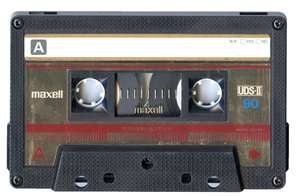
\includegraphics[scale=1.2]{pics/tape.eps} \\
\small
\verb+http://is.gd/3fp5Vx+
\end{center}
\Normalsize


\subsection{{\tt lseek(2)}}
\small
\setlength{\unitlength}{1mm}
\begin{center}
	\begin{picture}(230,30)
		\thinlines
		\put(0,0){\framebox(210,30){}}
		\put(10,25){{\tt \#include <sys/types.h>}}
		\put(10,20){{\tt \#include <fcntl.h>}}
		\put(10,12){{\tt off\_t lseek(int {\em filedes}, off\_t {\em offset}, int {\em whence} );}}
		\put(145,3){Returns:  new file offset if OK, -1 on error}
	\end{picture}
\end{center}
\Normalsize
\vspace{.25in}
The value of whence determines how offset is used:
\small
\begin{itemize}
	\item {\tt SEEK\_SET} bytes from the beginning of the file
	\item {\tt SEEK\_CUR} bytes from the current file position
	\item {\tt SEEK\_END} bytes from the end of the file
\end{itemize}
\Normalsize
\vspace{.25in}
``Weird'' things you can do using {\tt lseek(2)}:
\begin{itemize}
	\item seek to a negative offset
	\item seek 0 bytes from the current position
	\item seek past the end of the file
\end{itemize}

\subsection{{\tt lseek(2)}}
\begin{verbatim}
$ cc -Wall lseek.c
$ ./a.out < lseek.c
seek OK
$ cat lseek.c | ./a.out
cannot seek
$ mkfifo fifo
$ ./a.out <fifo

\end{verbatim}



\subsection{{\tt lseek(2)}}
\begin{verbatim}
$ cc -Wall hole.c
$ ./a.out
$ ls -l file.hole
-rw-------  1 jschauma  wheel  10240020 Sep 18 17:20 file.hole
$ hexdump -c file.hole
0000000   a   b   c   d   e   f   g   h   i   j  \0  \0  \0  \0  \0  \0
0000010  \0  \0  \0  \0  \0  \0  \0  \0  \0  \0  \0  \0  \0  \0  \0  \0
*
09c4000  \0  \0  \0  \0  \0  \0  \0  \0  \0  \0   A   B   C   D   E   F
09c4010   G   H   I   J
09c4014
$ cat file.hole > file.nohole
$ ls -ls file.*
   96 -rw-------  1 jschauma  wheel  10240020 Sep 18 17:20 file.hole
20064 -rw-r--r--  1 jschauma  wheel  10240020 Sep 18 17:21 file.nohole
\end{verbatim}

\verb+https://en.wikipedia.org/wiki/Sparse_file+ (not on e.g. HFS+)


\subsection{{\tt I/O Efficiency}}
Reviewing the program {\tt simple-cat.c} from the last class:
\begin{itemize}
	\item assumes that {\em stdin} and {\em stdout} have been set up
		appropriately
\end{itemize}

\subsection{{\tt I/O Efficiency}}
Reviewing the program {\tt simple-cat.c} from the last class:
\begin{itemize}
	\item assumes that {\em stdin} and {\em stdout} have been set up
		appropriately
	\item works for ``text'' and ``binary'' files since there is no such
		distinction in the UNIX kernel
\end{itemize}

\subsection{{\tt I/O Efficiency}}
Reviewing the program {\tt simple-cat.c} from the last class:
\begin{itemize}
	\item assumes that {\em stdin} and {\em stdout} have been set up
		appropriately
	\item works for ``text'' and ``binary'' files since there is no such
		distinction in the UNIX kernel
	\item how do we know the optimal {\tt BUFFSIZE}?
\end{itemize}

\subsection{{\tt I/O Efficiency}}
\begin{verbatim}
$ make tmpfiles

$ for n in $(seq 10); do
        dd if=/dev/urandom of=tmp/file$n count=204800
done

$ i=1; for n in 1048576 32768 16384 4096 512 256 128 64 1 ; do
        cc -Wall -DBUFFSIZE=$n simple-cat.c;
        i=$(( $i + 1 ));
        time ./a.out <tmp/file$i >tmp/file$i.copy;
done

$ make catio

$ stat -f "%k" tmp/file1 # stat -c "%o" tmp/file1
\end{verbatim}

Note: results vary depending on OS/filesystem.

\newpage
\vspace*{\fill}
\begin{center}
    \Hugesize
        So far, so good...\\ [1em]
    \hspace*{5mm}
    \blueline\\
    \hspace*{5mm}\\
	What questions do you have?
\end{center}
\vspace*{\fill}


\newpage
\vspace*{\fill}
\begin{center}
    \Hugesize
        Hooray! \\ [1em]
    \hspace*{5mm}
    \blueline\\
    \hspace*{5mm}\\
        5 Minute Break
\end{center}
\vspace*{\fill}


\subsection{File Sharing}
Since UNIX is a multi-user/multi-tasking system, it is conceivable (and
useful) if more than one process can act on a single file simultaneously. In
order to understand how this is accomplished, we need to examine some kernel
data structures which relate to files.  (See: Stevens, pp 75 ff)

\subsection{File Sharing}
Since UNIX is a multi-user/multi-tasking system, it is conceivable (and
useful) if more than one process can act on a single file simultaneously. In
order to understand how this is accomplished, we need to examine some kernel
data structures which relate to files.  (See: Stevens, pp 75 ff)

\begin{itemize}
	\item each process table entry has a table of file descriptors, which contain
		\begin{itemize}
			\item the file descriptor flags (e.g. {\tt FD\_CLOEXEC}, see \verb+fcntl(2)+)
			\item a pointer to a file table entry
		\end{itemize}
\end{itemize}

\subsection{File Sharing}
Since UNIX is a multi-user/multi-tasking system, it is conceivable (and
useful) if more than one process can act on a single file simultaneously. In
order to understand how this is accomplished, we need to examine some kernel
data structures which relate to files.  (See: Stevens, pp 75 ff)

\begin{itemize}
	\item each process table entry has a table of file descriptors, which contain
		\begin{itemize}
			\item the file descriptor flags (e.g. {\tt FD\_CLOEXEC}, see \verb+fcntl(2)+)
			\item a pointer to a file table entry
		\end{itemize}
	\item the kernel maintains a file table;  each entry contains
		\begin{itemize}
			\item file status flags (\verb+O_APPEND+, \verb+O_SYNC+, \verb+O_RDONLY+, etc.)
			\item current offset
			\item pointer to a vnode table entry
		\end{itemize}
\end{itemize}

\subsection{File Sharing}
Since UNIX is a multi-user/multi-tasking system, it is conceivable (and useful)
if more than one process can act on a single file simultaneously. In
order to understand how this is accomplished, we need to examine some kernel
data structures which relate to files.  (See: Stevens, pp 75 ff)

\begin{itemize}
	\item each process table entry has a table of file descriptors, which
		contain
		\begin{itemize}
			\item the file descriptor flags (e.g. {\tt FD\_CLOEXEC}, see \verb+fcntl(2)+)
			\item a pointer to a file table entry
		\end{itemize}
	\item the kernel maintains a file table;  each entry contains
		\begin{itemize}
			\item file status flags (\verb+O_APPEND+, \verb+O_SYNC+, \verb+O_RDONLY+, etc.)
			\item current offset
			\item pointer to a vnode table entry
		\end{itemize}
	\item a vnode structure contains
		\begin{itemize}
			\item vnode information
			\item inode information (such as current file size)
		\end{itemize}
\end{itemize}

\subsection{File Sharing}
\begin{center}
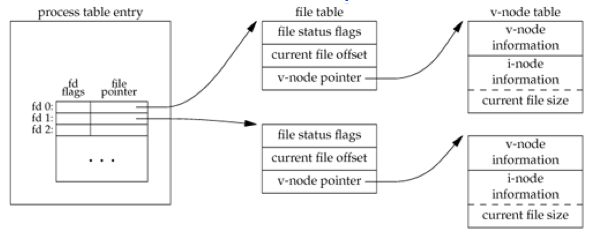
\includegraphics[scale=0.8,angle=-90]{pics/open-files.eps} \\
\end{center}

\subsection{File Sharing}
\begin{center}
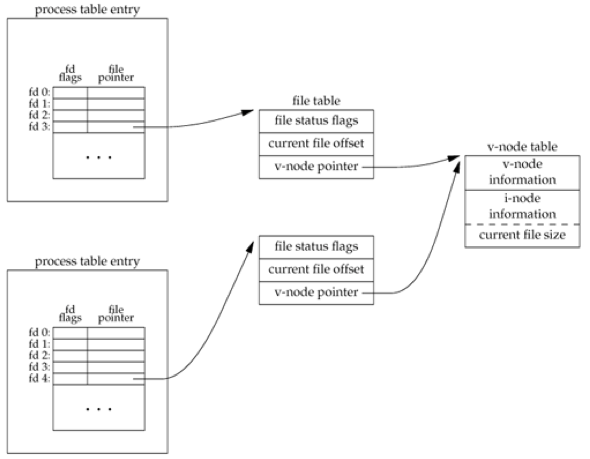
\includegraphics[scale=0.8,angle=-90]{pics/open-files-sharing.eps} \\
\end{center}


\subsection{File Sharing}
Knowing this, here's what happens with each of the calls we discussed earlier:

\begin{itemize}
	\item after each {\tt write} completes, the current file offset in the
		file table entry is incremented.  (If current\_file\_offset $>$
		current\_file\_size, change current file size in i-node table entry.)
	\item If file was opened {\tt O\_APPEND} set corresponding flag in file status
		flags in file table. For each {\tt write}, current file offset is first set to
		current file size from the i-node entry.
	\item {\tt lseek} simply adjusts current file offset in file table entry
	\item to {\tt lseek} to the end of a file, just copy current file size into
		current file offset.
\end{itemize}

\subsection{Atomic Operations}

In order to ensure consistency across multiple writes,
we require {\em atomicity} in some operations.  An
operation is atomic if either {\em all} of the steps
are performed or {\em none} of the steps are
performed.  \\

Suppose UNIX didn't have {\tt O\_APPEND} (early versions didn't). To
append, you'd have to do this:
\\

\small
\begin{verbatim}
if (lseek(fd, 0L, 2) < 0) {        /* position to EOF */
    fprintf(stderr, "lseek error\n");
    exit(1);
}

if (write(fd, buff, 100) != 100) { /* ...and write */
    fprintf(stderr, "write error\n");
    exit(1);
}
\end{verbatim}

\Normalsize

What if another process was doing the same thing to the same file? \\
Recall {\tt rwex.c}.

\subsection{{\tt pread(2)} and {\tt pwrite(2)}}
\small
\setlength{\unitlength}{1mm}
\begin{center}
	\begin{picture}(150,30)
		\thinlines
		\put(0,0){\framebox(130,30){}}
		\put(10,25){{\tt \#include <unistd.h>}}
		\put(10,17){{\tt ssize\_t pread(int {\em fd}, void *{\em buf}, size\_t {\em count}, off\_t {\em offset});}}
		\put(10,13){{\tt ssize\_t pwrite(int {\em fd}, void *{\em buf}, size\_t {\em count}, off\_t {\em offset});}}
		\put(45,3){Both return number of bytes read/written, -1 on error}
	\end{picture}
\end{center}
\Normalsize

Atomic read/write at offset without invoking {\tt lseek(2)}.

Current offset is {\em not} updated.


\subsection{{\tt dup(2)} and {\tt dup2(2)}}
\small
\setlength{\unitlength}{1mm}
\begin{center}
	\begin{picture}(150,30)
		\thinlines
		\put(0,0){\framebox(130,30){}}
		\put(10,25){{\tt \#include <unistd.h>}}
		\put(10,17){{\tt int dup(int {\em oldd});}}
		\put(10,12){{\tt int dup2(int {\em oldd}, int {\em newd});}}
		\put(55,3){Both return new file descriptor if OK, -1 on error}
	\end{picture}
\end{center}
\Normalsize

An existing file descriptor can be duplicated with {\tt dup(2)} or duplicated to
a particular file descriptor value with {\tt dup2(2)}. As with {\tt open(2)}, {\tt
dup(2)} returns the lowest numbered unused file descriptor.
\\

Note the difference in scope of the file {\em descriptor} flags and the
file {\em status} flags compared to distinct processes.
\begin{center}
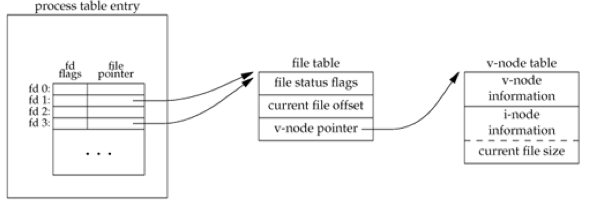
\includegraphics[scale=0.7,angle=-90]{pics/dup.eps} \\
\end{center}


\subsection{{\tt fcntl(2)}}
\small
\setlength{\unitlength}{1mm}
\begin{center}
	\begin{picture}(200,35)
		\thinlines
		\put(0,0){\framebox(180,35){}}
		\put(10,30){{\tt \#include <sys/types.h>}}
		\put(10,25){{\tt \#include <unistd.h>}}
		\put(10,20){{\tt \#include <fcntl.h>}}
		\put(10,12){{\tt int fcntl(int {\em filedes}, int {\em cmd}, ... /* int {\em arg} */);}}
		\put(110,3){Returns: depend on {\em cmd} if OK, -1 on error}
	\end{picture}
\end{center}
\Normalsize

{\tt fcntl(2)} is on of those "catch-all" functions with a myriad of purposes.
Here, they all relate to changing properties of an already open file. It can:
\vspace{.25in}

\begin{tabular}{l l l}
	{\bf cmd} & {\bf effect} & {\bf return value} \\
	\hline
	{\tt F\_DUPFD} & duplicate {\em filedes} \small({\tt FD\_CLOEXEC} file descriptor flag is cleared \Normalsize& new filedes \\
	{\tt F\_GETFD} & get the file descriptor flags for {\em filedes} & descriptor flags \\
	{\tt F\_SETFD} & set the file descriptor flags to the value of the third argument & not -1 \\
	{\tt F\_GETFL} & get the file status flags & status flags \\
	{\tt F\_SETFL} & set the file status flags & not -1
\end{tabular}
\vspace{.25in}

...as well as several other functions.

\subsection{{\tt fcntl(2)}}
\begin{verbatim}
$ cc -Wall sync-cat.c -o scat
$ sed -e 's/\(.*O_SYNC.*\)/\/\/\1/' sync-cat.c > async-cat.c
$ cc -Wall async-cat.c -o ascat
$ time ./scat <file >out

$ time ./ascat <file >out

$ make sync async

\end{verbatim}
\vspace{.25in}

Note: results will differ depending on the filesystem (-options).

\subsection{{\tt ioctl(2)}}
\small
\setlength{\unitlength}{1mm}
\begin{center}
	\begin{picture}(150,30)
		\thinlines
		\put(0,0){\framebox(130,30){}}
		\put(10,25){{\tt \#include <unistd.h>		/* SVR4 */}}
		\put(10,20){{\tt \#include <sys/ioctl.h>	/* 4.3+BSD */}}
		\put(10,12){{\tt int ioctl(int {\em filedes}, int {\em request}, ...);}}
		\put(55,3){Returns: -1 on error, something else if OK}
	\end{picture}
\end{center}
\Normalsize

Another catch-all function, this one is designed to handle device specifics
that can't be specified via any of the previous function calls. For example,
terminal I/O, magtape access, socket I/O, etc.

Mentioned here mostly for completeness's sake.

\subsection{{\tt /dev/fd}}
\begin{verbatim}
$ bash
$ ls -l /dev/stdin /dev/stdout /dev/stderr
lr-xr-xr-x  1 root  wheel  0 Sep  7 13:56 /dev/stderr -> fd/2
lr-xr-xr-x  1 root  wheel  0 Sep  7 13:56 /dev/stdin -> fd/0
lr-xr-xr-x  1 root  wheel  0 Sep  7 13:56 /dev/stdout -> fd/1
$ ls -l /dev/fd/
total 0
crw--w----   1 jschaumann  tty     16,   4 Sep  8 21:48 0
crw--w----   1 jschaumann  tty     16,   4 Sep  8 21:48 1
crw--w----   1 jschaumann  tty     16,   4 Sep  8 21:48 2
drw-r--r--  93 jschaumann  staff      3162 Sep  8 21:40 3
dr--r--r--   1 root        wheel         0 Sep  7 13:56 4
$ echo first >file1
$ echo third >file2
$ echo second | cat file1 /dev/fd/0 file2
\end{verbatim}

Note:
{\tt https://marc.info/?l=ast-users\&m=120978595414990\&w=2}


\subsection{Homework}
\begin{itemize}
	\item Reading:
		\begin{itemize}
			\item manual pages for the functions covered
			\item Stevens Chap. 3, 4
		\end{itemize}
	\item Thinking:
		\begin{itemize}
			\item Stevens \# 3.4
			\item Stevens \# 3.5 (bourne shell syntax ``$>\&$'')
			\item Use {\tt openat(2)} to protect against TOCTOU issues.
			\item Confirm that {\tt write(2)} clearing the setuid bit foils your evil attempts to root the system.
			\item Determine the optimal file I/O size on different systems via the benchmark example.
		\end{itemize}
	\item Coding:
		{\tt https://stevens.netmeister.org/631/f18-hw1.html}
\end{itemize}

\end{document}
